% Options for packages loaded elsewhere
\PassOptionsToPackage{unicode}{hyperref}
\PassOptionsToPackage{hyphens}{url}
%
\documentclass[
  12pt,
  ignorenonframetext,
  aspectratio=169,
]{beamer}
\usepackage{pgfpages}
\setbeamertemplate{caption}[numbered]
\setbeamertemplate{caption label separator}{: }
\setbeamercolor{caption name}{fg=normal text.fg}
\beamertemplatenavigationsymbolsempty
% Prevent slide breaks in the middle of a paragraph
\widowpenalties 1 10000
\raggedbottom
\setbeamertemplate{part page}{
  \centering
  \begin{beamercolorbox}[sep=16pt,center]{part title}
    \usebeamerfont{part title}\insertpart\par
  \end{beamercolorbox}
}
\setbeamertemplate{section page}{
  \centering
  \begin{beamercolorbox}[sep=12pt,center]{part title}
    \usebeamerfont{section title}\insertsection\par
  \end{beamercolorbox}
}
\setbeamertemplate{subsection page}{
  \centering
  \begin{beamercolorbox}[sep=8pt,center]{part title}
    \usebeamerfont{subsection title}\insertsubsection\par
  \end{beamercolorbox}
}
\AtBeginPart{
  \frame{\partpage}
}
\AtBeginSection{
  \ifbibliography
  \else
    \frame{\sectionpage}
  \fi
}
\AtBeginSubsection{
  \frame{\subsectionpage}
}
\usepackage{lmodern}
\usepackage{amssymb,amsmath}
\usepackage{ifxetex,ifluatex}
\ifnum 0\ifxetex 1\fi\ifluatex 1\fi=0 % if pdftex
  \usepackage[T1]{fontenc}
  \usepackage[utf8]{inputenc}
  \usepackage{textcomp} % provide euro and other symbols
\else % if luatex or xetex
  \ifxetex
    \usepackage{mathspec}
  \else
    \usepackage{unicode-math}
  \fi
  \defaultfontfeatures{Scale=MatchLowercase}
  \defaultfontfeatures[\rmfamily]{Ligatures=TeX,Scale=1}
\fi
\usetheme[]{Dresden}
\usecolortheme{dolphin}
\usefonttheme{structurebold}
% Use upquote if available, for straight quotes in verbatim environments
\IfFileExists{upquote.sty}{\usepackage{upquote}}{}
\IfFileExists{microtype.sty}{% use microtype if available
  \usepackage[]{microtype}
  \UseMicrotypeSet[protrusion]{basicmath} % disable protrusion for tt fonts
}{}
\makeatletter
\@ifundefined{KOMAClassName}{% if non-KOMA class
  \IfFileExists{parskip.sty}{%
    \usepackage{parskip}
  }{% else
    \setlength{\parindent}{0pt}
    \setlength{\parskip}{6pt plus 2pt minus 1pt}}
}{% if KOMA class
  \KOMAoptions{parskip=half}}
\makeatother
\usepackage{xcolor}
\IfFileExists{xurl.sty}{\usepackage{xurl}}{} % add URL line breaks if available
\IfFileExists{bookmark.sty}{\usepackage{bookmark}}{\usepackage{hyperref}}
\hypersetup{
  pdftitle={Statistical Thinking in Biology Research},
  pdfauthor={Terry Neeman},
  hidelinks,
  pdfcreator={LaTeX via pandoc}}
\urlstyle{same} % disable monospaced font for URLs
\newif\ifbibliography
\setlength{\emergencystretch}{3em} % prevent overfull lines
\providecommand{\tightlist}{%
  \setlength{\itemsep}{0pt}\setlength{\parskip}{0pt}}
\setcounter{secnumdepth}{-\maxdimen} % remove section numbering
\usepackage{fancyvrb}

\title{Statistical Thinking in Biology Research}
\subtitle{An introduction}
\author{Terry Neeman}
\date{30th July 2020}
\institute{Australian National University}

\begin{document}
\frame{\titlepage}

\begin{frame}{A few key ideas}
\protect\hypertarget{a-few-key-ideas}{}

\begin{itemize}
\tightlist
\item
  Statistics in biology is the study of biological variation
\item
  Understanding biological variation informs experimental design
\item
  Understanding biological variation informs data analysis
\end{itemize}

\begin{block}{Statistical thinking is an essential component of
scientific thinking}

\end{block}

\end{frame}

\begin{frame}{Some history of statistical methods in biology - 20th
century}
\protect\hypertarget{some-history-of-statistical-methods-in-biology---20th-century}{}

\begin{itemize}
\tightlist
\item
  Agricultural experiments in Rothamsted Station, UK
\item
  Stochastic processes in genetics
\item
  Clinical trials
\end{itemize}

\begin{figure}

{\centering 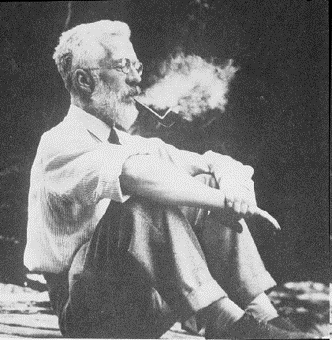
\includegraphics[width=0.3\linewidth,height=0.3\textheight]{../images/Lecture1_RA_Fisher} 

}

\caption{R.A. Fisher 1890 - 1962}\label{fig:unnamed-chunk-1}
\end{figure}

The ideas from these intellectual movements gave us foundations for how
we think about and interpret data as scientific evidence.

When teaching statistics, these ideas can get distilled, degraded into a
simplistic and false narrative.

\end{frame}

\hypertarget{some-false-narratives-cautionary-tales}{%
\section{Some false narratives (``cautionary
tales'')}\label{some-false-narratives-cautionary-tales}}

\begin{frame}{``Statistical analysis is all about getting a p-value''}
\protect\hypertarget{statistical-analysis-is-all-about-getting-a-p-value}{}

\begin{block}{Vaccine challenge experiment}

\begin{itemize}
\tightlist
\item
  6 mice per vaccine group (saline/ low dose / high dose)
\item
  All mice challenged with Shigella bacteria at Day 14
\item
  Outcome: 7-day average symptom score post-challenge
\end{itemize}

\begin{figure}

\hfill{}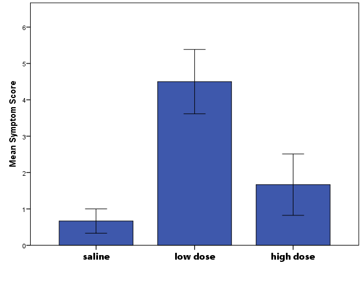
\includegraphics[width=0.5\linewidth,height=0.5\textheight]{../images/Lecture1_barplot} 

\caption{Mean Symptom Score, by Treatment}\label{fig:unnamed-chunk-2}
\end{figure}

\begin{block}{Statistical analysis: one-way ANOVA, p=0.04 post hoc
Bonferroni adjusted}

\end{block}

\end{block}

\end{frame}

\begin{frame}{Was there a cage effect or a vaccine effect?}
\protect\hypertarget{was-there-a-cage-effect-or-a-vaccine-effect}{}

The observed difference in symptom scores could be due to:

\begin{itemize}
\tightlist
\item
  animal cage
\item
  vaccine treatment
\end{itemize}

These two factors are \textbf{CONFOUNDED}. It is impossible to separate
out these two effects.

\begin{figure}

\hfill{}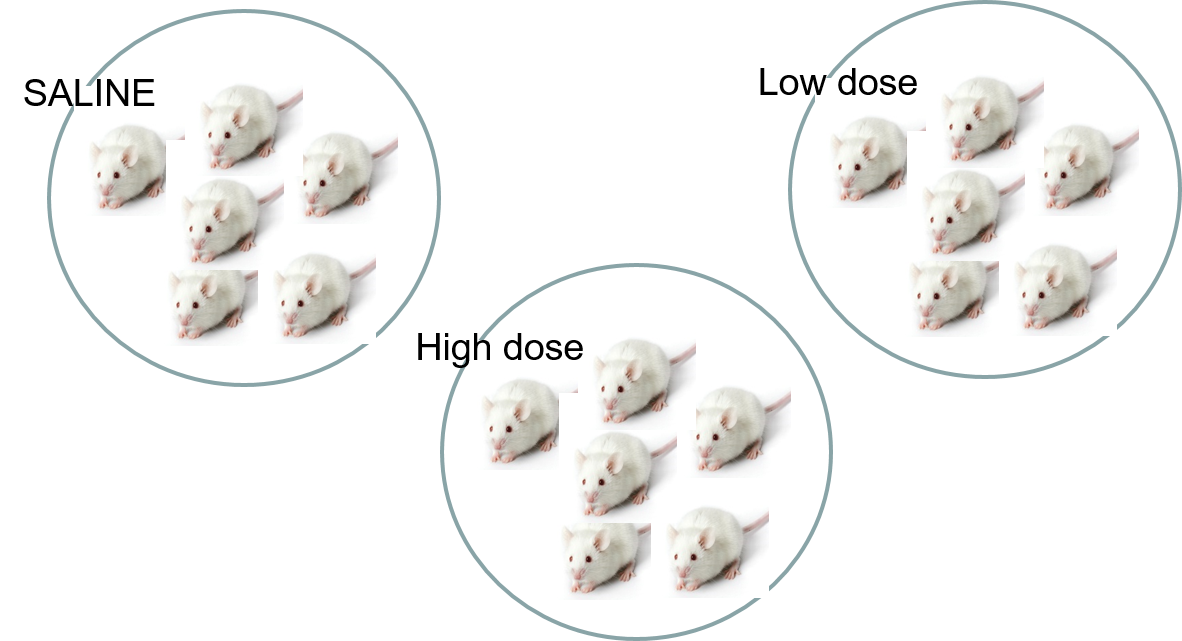
\includegraphics[width=0.5\linewidth,height=0.5\textheight]{../images/Lecture1_cages} 

\caption{Mean Symptom Score, by Treatment}\label{fig:unnamed-chunk-3}
\end{figure}

\begin{figure}

{\centering 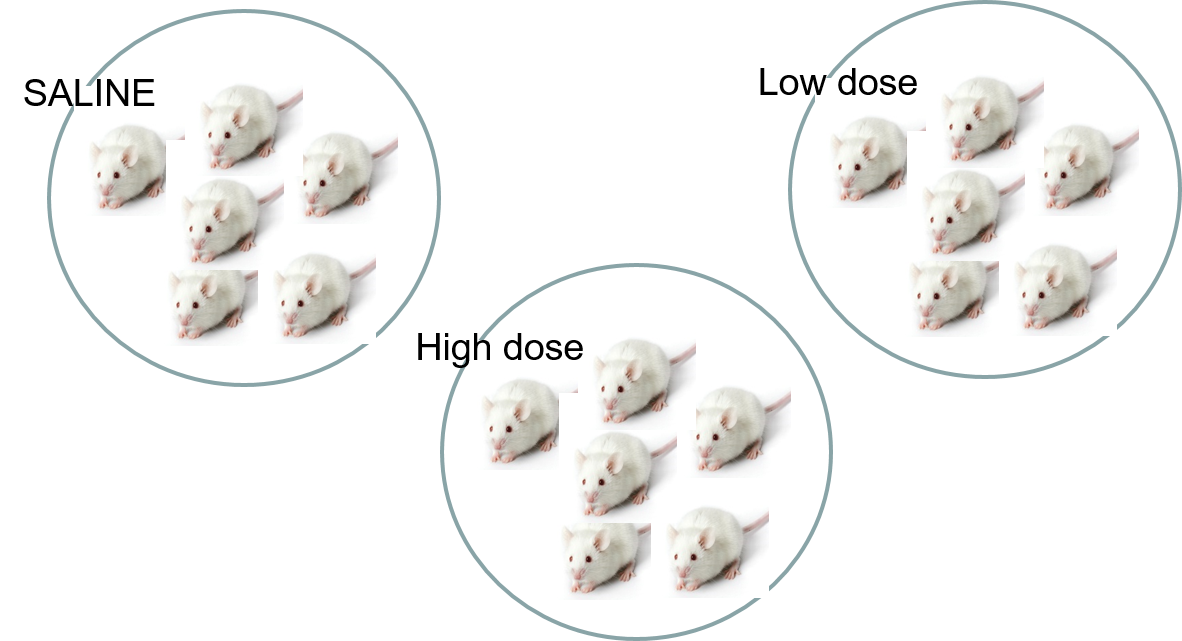
\includegraphics[width=0.5\linewidth,height=0.5\textheight]{../images/Lecture1_cages} 

}

\caption{Mean Symptom Score, by Treatment}\label{fig:unnamed-chunk-4}
\end{figure}

\end{frame}

\begin{frame}{``P \textgreater{} 0.05 means `same'; P \textless{} 0.05
means `different'\,''}
\protect\hypertarget{p-0.05-means-same-p-0.05-means-different}{}

Experimental set-up: Are temperature mechanisms modified in a
genetically-engineered tomato plant?

\begin{itemize}
\tightlist
\item
  Genotypes: WT or mutant
\item
  watering conditions: normal or drought
\item
  Outcome: leaf temperature at 7 days post-treatment
\end{itemize}

\begin{figure}

\hfill{}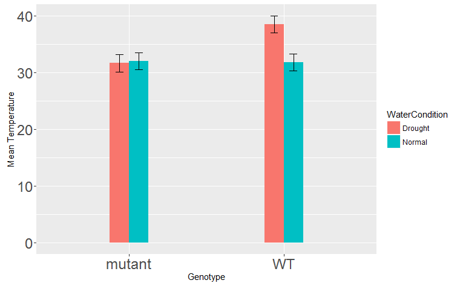
\includegraphics[width=0.4\linewidth,height=0.4\textheight]{../images/Lecture1_interaction} 

\caption{Leaf temperature under different watering conditions}\label{fig:unnamed-chunk-5}
\end{figure}

\end{frame}

\begin{frame}{``When in doubt, use lots of t-tests''}
\protect\hypertarget{when-in-doubt-use-lots-of-t-tests}{}

Research questions: Are mice susceptible to obesity when exposed to a
high fat diet? Are NODk mice \textbf{MORE} susceptible than mice without
mutation?

\begin{center}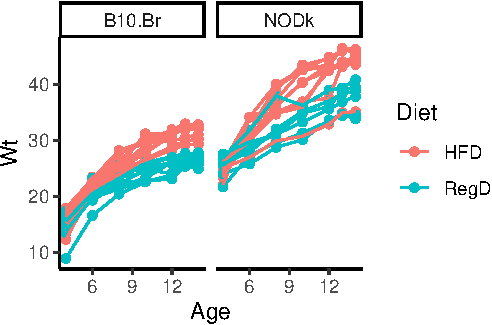
\includegraphics{Lecture-1_files/figure-beamer/unnamed-chunk-6-1} \end{center}

\end{frame}

\begin{frame}{``More than 2 groups? Use 1-way ANOVA''}
\protect\hypertarget{more-than-2-groups-use-1-way-anova}{}

Research question: Which barley variety has the biggest yield?

\begin{itemize}
\tightlist
\item
  Five barley varieties, grown in 6 locations
\item
  Two growing seasons
\item
  Outcome: yield (tonnes/hectare)
\end{itemize}

\begin{center}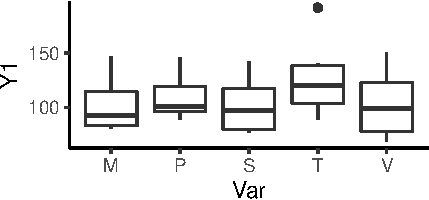
\includegraphics{Lecture-1_files/figure-beamer/unnamed-chunk-7-1} \end{center}

\end{frame}

\begin{frame}{Location contributes to the variation in yield}
\protect\hypertarget{location-contributes-to-the-variation-in-yield}{}

\begin{center}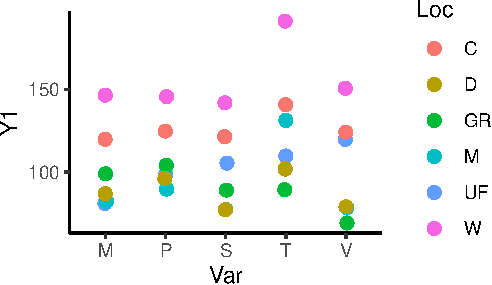
\includegraphics{Lecture-1_files/figure-beamer/unnamed-chunk-8-1} \end{center}

Yield is highest in Locations C and W. Yield is lowest in Locations D
and GR.

\end{frame}

\begin{frame}{Varieties should be compared \emph{within} location}
\protect\hypertarget{varieties-should-be-compared-within-location}{}

\begin{center}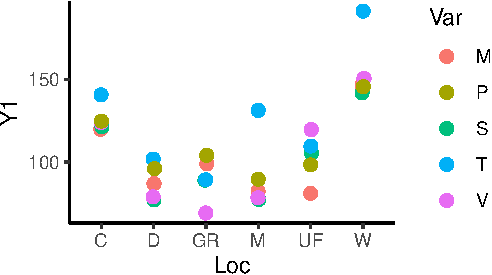
\includegraphics{Lecture-1_files/figure-beamer/unnamed-chunk-9-1} \end{center}

Notice that: Variety M is near the bottom in most locations\\
Variety T is near the top in most locations

\end{frame}

\begin{frame}{``When I see a scatterplot, I fit a linear regression''}
\protect\hypertarget{when-i-see-a-scatterplot-i-fit-a-linear-regression}{}

Ecology researchers recorded \textbf{density of thorn-like plants} in
multiple locations across five regions, and measured \textbf{per hectare
consumption} of plant material by herbivores.

\begin{center}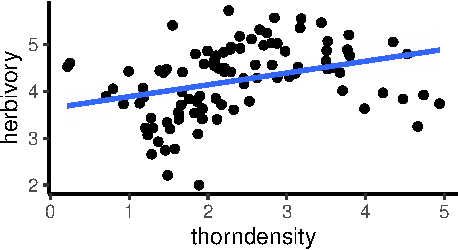
\includegraphics{Lecture-1_files/figure-beamer/unnamed-chunk-10-1} \end{center}

\end{frame}

\begin{frame}{Herbivory vs Thorns, by Site}
\protect\hypertarget{herbivory-vs-thorns-by-site}{}

Ecology researchers recorded \textbf{density of thorn-like plants} in
multiple locations across \textbf{five sites}, and measured \textbf{per
hectare consumption} of plant material by herbivores.

\begin{center}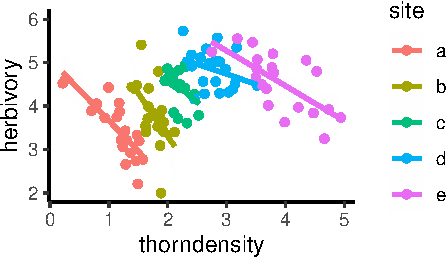
\includegraphics{Lecture-1_files/figure-beamer/unnamed-chunk-11-1} \end{center}

\end{frame}

\begin{frame}{Summary}
\protect\hypertarget{summary}{}

\begin{itemize}
\item
  Message 1: Building a scientific case for a treatment effect is not
  just about the p-value. Must understand the context of experiment(s).
\item
  Message 2: P-values from simple contrasts cannot tell us if the
  contrasts are different.
\item
  Message 3: Interpreting experimental results needs more than t-tests.
\item
  Message 4: We need to incorporate known sources of variation into
  statistical analyses.
\item
  Message 5: What's more important than p-values and t-tests?

  \begin{itemize}
  \tightlist
  \item
    recognising patterns in data
  \item
    understanding sources of variation
  \item
    useing data to build information about complex systems
  \item
    using statistics to allow the data to speak
  \end{itemize}
\end{itemize}

\end{frame}

\end{document}
